\documentclass[11pt,a4paper]{article}
\usepackage[utf8]{inputenc}
\usepackage[T1]{fontenc}
\usepackage{amsmath,amsfonts,amssymb}
\usepackage{apacite}
\usepackage{natbib}
\usepackage{graphicx}
\usepackage{booktabs}
\usepackage{threeparttable}
\usepackage{url}
\usepackage{hyperref}
\usepackage[margin=2.5cm]{geometry}
\usepackage{setspace}
\usepackage{comment}
\usepackage{outlines}
\onehalfspacing

\newcommand{\Var}{\text{Var}}
\newcommand{\Cov}{\text{Cov}}

% Define \sym command for significance stars from esttab
\newcommand{\sym}[1]{{#1}}

\title{CEOs and Firm Performance: Estimation from the Universe of Firms\thanks{Project no. 144193 has been implemented with the support provided by the Ministry of Culture and Innovation of Hungary from the National Research, Development and Innovation Fund, financed under the KKP\_22 funding scheme. This project was funded by the European Research Council (ERC Advanced Grant agreement number 101097789). Telegdy received support from the Hungarian Scientific Research Fund – OTKA, contract number 143346. The views expressed in this research are those of the authors and do not necessarily reflect the official view of the European Union or the European Research Council. \emph{Author contributions:} Conceptualization and study design: Koren, Orbán and Telegdy. Data curation, integration and quality assurance: Szilágyi and Vereckei. Statistical analysis: Koren, Orbán and Telegdy. Writing the original draft: Koren. Review and editing: Koren, Orbán and Telegdy.}}

\author{Miklós Koren\thanks{Central European University, ELTE Centre for Economic and Regional Studies, CEPR and CESifo. E-mail: korenm@ceu.edu} \\
        Krisztina Orbán\thanks{Monash University.} \\
        Bálint Szilágyi\thanks{ELTE Centre for Economic and Regional Studies.} \\
        Álmos Telegdy\thanks{Corvinus University of Budapest.} \\
        András Vereckei\thanks{ELTE Centre for Economic and Regional Studies, Institute of Economics.}}

\date{September 2025}

\begin{document}

\maketitle
\thispagestyle{empty}

\begin{abstract}
How much do CEOs matter for firm performance? We estimate the causal effect of CEO quality on productivity using comprehensive administrative data covering the universe of Hungarian firms and CEOs from 1992--2022. We develop a production function framework that separates owner-controlled strategic decisions from CEO-controlled operational decisions. To address the severe measurement error in CEO fixed effects arising from short tenures, we introduce a placebo-controlled event study design: we compare actual CEO transitions to randomly assigned fake transitions in firms with stable leadership. The results reveal that a CEO better than the incumbent increases firm performance by 3\% while a worse CEO decreases it by 2\%. CEO changes contribute to the variance growth of productivity by 30\% in the first 10 years of the firm's existence. The placebo-controlled methodology provides a general solution for estimating individual effects in short-panel settings.
\end{abstract}

\textbf{Keywords:} CEO value, private firms, productivity

\textbf{JEL Classification:} D24, G34

\clearpage
\setcounter{page}{1}

%%%%%%%%%%%%%%%%%%%%%%
\section{Introduction}
%%%%%%%%%%%%%%%%%%%%%%

%Why are CEOs important?
To what extent do CEOs contribute to firm performance? Good management can improve firm productivity, as suggested by studies analyzing leadership changes \citep{Bertrand2003-io,bennedsen2020ceos,metcalfe2023managers}, by intervention studies improving management practices \citep{bloom2013does} and training programs for managers \citep{mckenzie2021small, bianchigiorcellitraining}.

%what we do
In this paper, we analyze the impact of CEOs on firm productivity. We make three contributions to the literature. First, we develop a model that accounts for the division of control between owners and managers. Second, we assemble a dataset based on two administrative databases covering the universe of Hungarian firms and their CEO networks over three decades (1992-2022). Third, we employ a regression design which uses firm and CEO fixed effects (in the spirit of \cite{abowd1999high}) to uncover the contribution of CEOs to firm productivity; this approach has been used since the beginning of this strand of literature \citep{Bertrand2003-io}. We improve on this estimation framework by introducing a placebo-controlled event study design that separates true CEO effects from the mechanical noise that contaminates firm and manager fixed effects estimates in the presence of limited mobility bias and short managerial spells. We also perform a decomposition of the variance to quantify the impact of CEOs on firm productivity.

%Why is our approach unique - model
Our modeling approach specifies the role of owners and CEOs in operational decisions. Owners set fixed inputs (such as tangible and intangible capital) and CEOs optimize variable inputs (labor, materials). This simplification underestimates CEOs' strategic importance, but it has two advantages. First, it does not attribute all the effects of capital to the CEO as owners -- the providers of capital -- are naturally the final decision makers in this respect.\footnote{Even if the firm is founder managed (so the owner and the CEO are identical), family interests and financial constraints will impede the smooth changes in the capital structure.} Second, we argue that by making the owner the sole decision maker regarding capital, our estimation of the CEO effects on firm productivity will be downward biased because as capital will be controlled for in the regressions.\footnote{As we will show later, firms under good CEOs grow and have more capital. Controlling for capital reduces the effect of CEOs, even if part of the capital is correlated with their ability.}

%Why is our approach unique - data
Papers use three approaches when analyzing the effect of CEOs. One group studied the effects of a distinct, measurable variable, such as managerial practices used in the firm \citep{bloom2012organization} or a CEO attribute (age, gender, tenure, education or country of origin \citep{anderson2018pathways, henderson2006quickly, Koren2023expat}). These studies are useful to show the effects of the studied variables, but they arguably capture little of the whole effect of CEOs over the firms they manage. Another group uses an external event to assess the effect of CEO turnover (e.g., \citet{bennedsen2020ceos}). While this approach brought about credible causal estimates, the heavy data needs render this approach impossible to use in most situations. 

The third group employed firm and CEO fixed effects to separate the quality of firm from that of the CEOs \citep{Bertrand2003-io, crossland2011differences, quigley2015has}. While these studies employ a framework that can be used in many settings, the generalizability of their results is challenged by the data used because almost all study public companies only.\footnote{\citet{quigley2022ceo} is a notable exception studying CEO effects in private businesses, but the private sample comprises of large firms.} Our data has information on the universe of Hungarian businesses and all their CEOs for the period between 1992 and 2022, tracking over 1 million firms and a similar number of CEOs.\footnote{Mandatory registration of all company directors ensures complete coverage of CEOs in the whole corporate sector.} The overwhelming majority of the firms in our sample are small and medium-sized enterprises (SMEs). This adds a new dimension to the analysis that was largely missing from the literature and allows drawing conclusions about CEOs' effects on the whole economy. Our analysis is also distinctive in that earlier studies focused on developed countries, while our data come from Hungary. Indeed, the institutional context matters: \citet{crossland2011differences} show that informal and formal institutions affect CEO discretion.

%Why is our approach unique - estimation
%Our goal is to relate CEOs to firm productivity, and our model helps separating the part of the productivity which is attributed to the CEO from the contribution of capital to productivity, which we attribute to the owner. For this, we need to compute the surplus share of the cost of materials and labor in revenue. We do this by computing this variable from the firm-level data for separate sectors. We also need to estimate the elasticity of revenue with respect to capital. This is computed with the help of our estimable revenue function derived from the model. [[K: i think this is not true: will think about ti later.]] As we include CEO and firm fixed effects to this regression, we do not require exogenous mobility to obtain an unbiased capital elasticity. Good CEOs may sort together with good firms. All we need is that productivity shocks do not coincide with CEO replacement. Having obtained the short run productivity of the firm, we deconstruct it into manager-specific skill, firm effects, and residual noise. 

Our model produces a measure of firm productivity that is directly dependent on the CEO. Firm productivity is the dependent variable in our baseline regression, where we correlate productivity with firm and CEO fixed effects. We define the value of each CEO as the average firm productivity measured over all firm-years when the CEO was in office.

While the estimation of CEO effects is unbiased under standard identification assumptions of fixed effects regressions, bias may arise when regressions are conducted on subsamples segmented by CEO quality. (Estimating the effect of CEO quality on firm performance is the ultimate goal of such studies.) This is caused by the short time span of many CEOs and also by the fact that we observe few CEO replacements for a firm.\footnote{This is the limited mobility bias, which contaminates the second moment of wage regressions in the presence of worker and firm fixed effects \cite{kline2024firm}.} CEO fixed effects are estimated from few changes and CEO and firm fixed effects will partly overlap. Firms that experience a positive shock will be more likely classified as having good CEOs, and those that draw a negative shock as having bad CEOs. To address this bias, we introduce a placebo-controlled event study design.

The main idea of this correction is the creation of pseudo CEO transitions in the data\footnote{This step in the spirit of \cite{jarosiewicz2023revisiting}, who compare the replicated results of  \cite{Bertrand2003-io} with placebo regressions.} We take firms with CEO transitions, record their event window. The event window is the period encompassing the years under the CEO prior to the CEO change and the period under the new CEO post the change. We match these firms to firms born in the same year, belonging to the same sector, that however do not experience a CEO transition during the years of the event window. Then, we assign to the control firms a placebo CEO transition happening in the same year as the treated firm experiences the true CEO transition.\footnote{In addition to addressing the limited mobility bias, our approach has the advantage of creating a control group that is more similar to the treated firms than the universe of firms}. On the matched sample we implement two-way fixed effects regressions.\footnote{The estimation is similar to the two way fixed effects regression developed by \cite{Callaway2021JoLE}, but we exploit the fact that the control group also has a time of pseudo CEO change. We compare firms with a true CEO change with firms with a fake CEO change along the same event-time years.} If estimated `effects' for these pseudo-CEOs diverge substantially, this reveals the noise problem in fixed effects estimation. By comparing actual CEO transitions to these placebo transitions, we can correct the fixed effects estimates for noise, isolating the true CEO contribution.

%results
Our results indicate that the average CEO transition does not have substantial effects on firm productivity. This result is not counterintuitive: sorting by quality implies that CEO replacements tend to be matched with successors of comparable quality. Nonetheless, sorting is not perfect and we find large swings in productivity when we run the regression for transitions that improve or decline CEO quality.\footnote{In these regression, we also select the control sample by improving and declining productivity along the pseudo CEO transition.} Our placebo-controlled regressions estimate a 3\% increase in productivity when the CEO value increases, and a 2\% decline when it decreases. The low magnitude is due to our correction mechanism: in the placebo estimates, the measured ``effect'' is on the order of 20\%.  

To validate our model, we run the same regressions on the main inputs of the firm. Contrary to our assumption about capital not being affected by CEOs, we find that the value of tangible assets declines before, and increases after the CEO change, but the proportion of firms possessing intangible capital does not change. However, the change in tangible assets is both smaller and slower than the massive change which are measured for both short term inputs, the cost of materials and labor. While the change in tangible assets is 5-10\%, variable inputs change by about 20\% in an order of magnitude larger.

To quantify the effect of CEOs on firm performance in our data, we perform a variance decomposition, which computes what proportion of the total dispersion of productivity change is explained by CEO transitions. As demonstrated by countless papers in labor economics, the variance is also contaminated by the limited mobility bias and we make a correction of it with the  placebo method. With our carefully chosen control group we also take into account the mechanical effect of firm age on productivity dispersion: as time passes, the firm gathers shocks and so the dispersion will increase. 

We find that CEO transitions explain about 30\% of the productivity change in our data. The placebo correction is also important here: without it, this share would be about twice as large.

%literature
Our work connects to the broader literature on management practices and firm productivity. Randomized controlled trials demonstrate that management training and consulting improve firm performance \citep{bloom2013does, mckenzie2021small}, but these interventions change practices rather than people. Whether replacing managers generates similar gains remains contentious. Evidence from public sector organizations suggests modest manager effects \citep{fenizia2022managers, janke2024role}, while studies of family firms find larger impacts when professional managers replace family members \citep{bennedsen2007inside, sraer2007performance}. Our results for private firms fall between these extremes: CEOs matter, but less than raw correlations suggest.

Methodologically, our paper builds on the two-way fixed effects literature in labor economics that decomposes wages into worker and firm components \citep{Abowd1999Econometrica, Card2018JoLE}. These studies face similar challenges from limited mobility creating small-sample bias \citep{andrews2008high} and have developed bias-correction methods \citep{Bonhomme2023-dx, gaure2014correlation}. We adapt this framework to the CEO-firm setting but add placebo controls to separate signal from noise. This approach is valuable when studying managers who, unlike workers, have few observations per individual, making traditional bias-correction methods less effective. Recent work has documented apparently increasing CEO effects over time \citep{quigley2015has}, but these studies do not account for the mechanical noise we identify. \citet{lippi2014corporate} find that concentrated ownership in Italian firms distorts executive selection and reduces productivity by 10\%, providing motivation for our framework separating owner and CEO decisions.

%%%%%%%%%%%%%%%%%%%%%%%%%%%%%%%%%%
\section{A Model of Production with Owner- and Manager-Controlled Inputs}
%%%%%%%%%%%%%%%%%%%%%%%%%%%%%%%%%%%

In this section we develop a simple model of firm production to establish how CEOs contribute to firm productivity. An important feature of this model is that CEO skill is a direct component of TFP, but is also correlated with input choice: under skilled managers firms will purchase more inputs due to the complementarity of productivity and inputs. 

In the model, we attribute decisions regarding short run inputs as labor and material to the CEO while investment is decided by the owner.\footnote{We abstract from agency problems between the owner and the CEO.} While this is probably too restrictive regarding the role of the CEO in long-run investment, we do this for three reasons. First, there is no theoretical guidance on the process of decision making regarding investment, especially among private firms. Second, we estimate the effect of CEOs on productivity around a CEO replacement which is a short-run effect by construction and capital is likely to change in the longer run. Third, modeling capital as fixed from the perspective of the CEO will result in a downward bias of CEOs on productivity, as good CEOs will often be observed as working with higher levels of capital. 

We define a Cobb-Douglas production function with both fixed and variable inputs. The production function for firm $i$ with manager $m$ at time $t$ is:
\begin{equation}\label{eq:production}
Q_{imt} = A_i Z_{m} \varepsilon_{it} K_{it}^\alpha L_{imt}^{\beta} M_{imt}^{\gamma}
\end{equation}
where $A_i$ represents time-invariant organizational capital (including items as location, brand value, customer relationships), $Z_m$ captures CEO skill, $K_{it}$, $L_{imt}$ and $M_{imt}$ are capital, labor and intermediate inputs, and $\varepsilon_{it}$ is the residual productivity. In standard production function estimation, total factor productivity (TFP) represents the first three components of the production function: $\Omega_{it} = A_i Z_m \varepsilon_{it}$. Our framework decomposes TFP into firm-specific components ($A_i$), manager-specific skill ($Z_m$), and residual productivity shocks ($\varepsilon_{it}$) to identify the manager contribution. The production function exhibits decreasing returns to scale in variable inputs ($\beta + \gamma < 1$), which pins down optimal firm size even under perfect competition. 

We assume physical capital investment ($K_{it}$) and organizational assets ($A_i$) are predetermined from the perspective of the CEO, who thus controls only labor ($L_{imt}$) and input purchases ($M_{imt}$). 

Managers maximize profit by choosing variable inputs optimally given the predetermined choices. Under sector-specific output price $P_{st}$, wage rate $W_{st}$, and material price $\varrho_{st}$, the first-order conditions yield closed-form solutions for optimal input demands. Substituting these back into the revenue function gives:
\begin{equation}\label{eq:revenue}
R_{imst} = (P_{st}A_i Z_m \varepsilon_{it})^{1/\chi}
K_{it}^{\alpha/\chi}
W_{st}^{-\beta/\chi}
\varrho_{st}^{-\gamma/\chi}
(1-\chi)^{(1-\chi)/\chi}
\end{equation}
Revenue increases in manager skill $Z_m$, organizational capital $A_i$, and physical capital $K_{it}$, while decreases in input prices. The elasticity of revenue with respect to manager skill is $1/\chi > 1$, with $\chi := 1 - \beta - \gamma$, the share of surplus in revenue. 

The surplus accruing to fixed factors ($K_{it}$ and everything embedded in $A_i$ and $Z_m$), equals revenue minus payments to variable inputs:
\begin{equation}\label{eq:surplus}
S_{imst} = R_{imst} - W_{st}L_{imt} - \varrho_{st}M_{imt} = \chi R_{imst}
\end{equation}
Under Cobb-Douglas technology, surplus is a constant fraction $\chi$ of revenue. This proportionality allows us to work directly with revenue, simplifying estimation while preserving economic insights. 

Taking logarithms of the revenue equation (\ref{eq:revenue}):
\begin{equation}\label{eq:log_revenue}
r_{imst} = C+\frac{\alpha}{\chi} k_{it} + \frac{1}{\chi} z_{m} + \frac{1}{\chi} a_i + \frac{1}{\chi} p_{st} - \frac{\beta}{\chi} w_{st} - \frac{\gamma}{\chi} \rho_{st} + \frac{1}{\chi}\epsilon_{it}
\end{equation}
where lowercase letters denote logarithms (e.g., $\epsilon_{it} = \log \varepsilon_{it}$) and $C$ is a constant.

The value of replacing manager $m$ with manager $m'$ at the same firm is the extent to which surplus changes as the manager changes:
\begin{equation}\label{eq:manager_value}
r_{im'st} - r_{imst} = \frac{1}{\chi}(z_{m'} - z_{m})
\end{equation}
The value difference between two CEOs of a firm is measured by the difference in firm revenue, and it equals the skill difference scaled by $1/\chi$. This scaling reflects a leverage effect: a 1\% better manager hires more variable inputs, thereby increasing revenue and surplus by more than 1\%.

The model excludes dynamic considerations such as adjustment costs or forward-looking behavior. Strategic decisions are forward-looking due to their persistence, but we treat them as predetermined from the manager's perspective. Even though the optimization framework is static, our empirical application allows for arbitrary time-series correlation within and across variables. The data validate this choice: strategic variables like capital evolve slowly with little correlation to manager changes, while operational variables adjust immediately following CEO transitions.

%%%%%%%%%%%%%%%%%%%%
\section{Estimation}\label{sec:est}
%%%%%%%%%%%%%%%%%%%%

Our estimation proceeds in four steps: we measure the surplus share $\chi$ (the share of revenue accruing to fixed factors), estimate the revenue function, recover manager fixed effects, and recover the dynamics of the estimated effects through event studies. Each step builds toward separating true CEO effects from the noise that contaminates raw estimates.

Having estimated the placebo-corrected CEO effect, we decompose the variance of TFP into a general component and one depending on the CEO. The share of the CEO dependent component in the total variance provides a quantification of the CEO effect on firm productivity.

\paragraph{Step 1: Measuring the Surplus Share.} The parameter $\chi$---the share of surplus in revenue---determines how manager skill translates into firm performance. Under Cobb-Douglas technology, this share equals one minus the combined revenue shares of labor and materials. Following \citet{Gandhi2020-nu}, we measure $\chi$ from the data as:
\begin{equation}
\hat{\chi}_s = 1 - \frac{\sum_{i \in s}(W_{st}L_{it} + \varrho_{st}M_{it})}{\sum_{i \in s} R_{it}}
\end{equation}
where the summation runs over firms in sector $s$. This approach yields sector-specific estimates of $\chi$. The $1/\chi$ scaling in our framework creates a leverage effect, amplifying the impact of managerial skill on firm performance.

\paragraph{Step 2: Estimating the Revenue Function.} With $\hat{\chi}$ in hand, we estimate the revenue function to recover the capital elasticity and control for observable factors. With an estimate of $\alpha_s/\chi_s$ recovered, we multiply it by $\hat{\chi_s}$ to recover $\hat{\alpha_s}$. Using lowercase letters for logarithms, the estimating equation is the empirical counterpart of (\ref{eq:log_revenue}):
\begin{equation}
r_{it(m,s)} = \frac{\alpha_s}{\chi_s} k_{it} + \frac{1}{\chi_s}z_m + \frac{1}{\chi_s} \lambda_i + \frac{1}{\chi_s} \mu_{st} + \tilde{\epsilon}_{it}
\end{equation}
where $r_{it(m,s)} = \log R_{imst(m,s)}$ is log revenue, $k_{it} = \log K_{it}$ is log capital, $\lambda_i$ captures firm fixed effects, $\mu_{st}$ are sector-year fixed effects, and $\tilde{\epsilon}_{it} = \epsilon_{it}/\chi$ is rescaled residual productivity. We estimate $\alpha/\chi$ in two ways: (a)  using GMM invoking a moment condition according to which the level of capital determined in the previous period is orthogonal to the error term in first differences  $E[k_{it} \Delta \tilde{\epsilon}_{it}]$; (b) as in (a) but adding additional controls such as firm age, intangible asset presence, foreign ownership.\footnote{Since capital is determined in period t-1, strict exogeneity does not hold, as such standard fixed effect estimators cannot be used in this step.} The estimated coefficients on capital differ only marginally.



The key assumptions to obtain a consistent estimate of $\alpha/\chi$ are: (1) all firms within a sector face the same prices, and (2) capital is decided in period t-1, and (3) the error term in t, purged from shocks observable to the firm but not the econometrician is uncorrelated with capital choice in t-1, $k_t$. 



\paragraph{Step 3: Recovering Manager Fixed Effects.} After estimating the revenue function, we compute log total factor productivity by removing the contribution of capital and sectoral prices from revenue:
\begin{equation}
\omega_{imst} = \hat{\chi} r_{imst} - \hat{\alpha} k_{it} - \hat{\mu}_{st} = z_m +  \lambda_i + \epsilon_{it}
\end{equation}
This measure of log TFP contains manager skill, firm effects, and residual productivity. In standard production function estimation, this entire term would be treated as a single TFP measure. Our decomposition separates the manager contribution from other sources of productivity.

We estimate a two-way fixed effects model with firm and manager fixed effects. Our identification relies on the strict exogeneity assumption where the conditional expectation of the error term $\epsilon_{it}$ is zero for a given firm-manager pair, for every t: $E[\epsilon_{it}|\lambda_i, z_m]=0$ for $t=1...T$ This assumption allows for various forms of endogenous mobility but rules out systematic patterns where managers consistently join improving or declining firms. The estimated CEO fixed effects are unbiased, but inconsistent due to the fact that with the sample size $N$ increasing, the length of tenure of CEO-s at a given firm does not increase.

The event study provides a diagnostic test for this identification assumption. Pre-trends in productivity before CEO transitions would suggest that the strict exogeneity assumption is violated. If productivity systematically rises before good CEOs arrive, we worry that the positive trend continues post-transition, violating $E[\epsilon_{it}|z_m, \lambda_i] = 0$ for $\forall t$. Conversely, the absence of pre-trends makes it harder to construct plausible endogeneity stories. While we cannot rule out contemporaneous shocks that coincide exactly with CEO changes (e.g., owners simultaneously firing the CEO and adopting new technology), such precise timing is less plausible than gradual changes that would manifest as pre-trends. Our event studies show no significant pre-trends, supporting but not proving our identification assumption.\footnote{The absence of strong pre-trends in our data contrasts with evidence from \citet{cornelli2013monitoring} showing boards actively monitor and replace CEOs when performance deteriorates in public firms, suggesting our private firm transitions may be less performance-driven. While \citet{jenter2021performance} find 38-55\% of turnovers are performance-induced in U.S. public firms, our private firm setting likely features more random CEO transitions given the absence of market pressures and board oversight.}

The system of fixed effects is identified only within connected components: groups of firms and managers linked through mobility. Two managers can be compared if they worked at the same firm or are connected through a chain of shared CEO-firm relationships. We can estimate $\hat z_m$ for every manager, but only up to a constant term that may vary across connected components. Our largest connected component contains 22,001 managers, enabling comparisons within this network. We normalize the manager effect to be mean zero in the largest connected component.
In TWFE models researchers are typically limited to analysis within the largest connected component of their network. We are not limited by the largest connected component, only by the set of firms which experience a CEO transition. 
As ours is a within firm analysis, the two CEO-s we compare at the event of a CEO transition always belong to the same connected component, and hence their estimated fixed effects are comparable.
\paragraph{Step 4: Placebo-Controlled Event Studies.} Even when $\epsilon$ is orthogonal to $z$, estimated fixed effects contain substantial small-sample noise when manager transitions are infrequent and manager tenures are short.\footnote{Worker-firm fixed effect studies face similar challenges called ``limited mobility bias'' \citep{andrews2008high}. This literature has developed bias-correction methods for the variance estimates of fixed effects \citep{Bonhomme2023-dx, gaure2014correlation}.} A consequence of this small sample bias is that naively estimating the effect of CEO transitions on TFP will likely overestimate the true effect.

To understand the sources of small-sample bias and how we address it, we remove the firm fixed effect from TFP by subtracting the firm average:
\begin{equation}
\Delta\omega_{imt} = \Delta z_{m_{it}} + \Delta\epsilon_{it},
\end{equation}
where $\Delta x_{it} := x_{it} - \frac{1}{N_i}\sum_{\tau} x_{i\tau}$ denotes the deviation of a variable from its within-firm mean. When a firm changes CEOs, the change in log TFP captures both the true skill difference and accumulated noise. The noise component---the average of residual productivity shocks during each manager's tenure---dominates the signal when tenures are short. 

Our solution leverages a simple insight: when CEOs do not change, we still observe variation in log TFP driven purely by noise:
\begin{equation}
\Delta\omega_{imt} = \Delta\epsilon_{it}.
\end{equation}
By applying the estimation procedure to measure the effect of CEO transitions on productivity not only to real CEO transitions but also to placebo CEO transitions, we can measure and filter out the noise component.

We construct placebo CEO transitions to use as control transitions to actual CEO transitions in three steps. First, we identify the set of clean CEO transitions by looking at firms with one CEO per year, where firms have at least two consecutive CEO spells. From around 3.5 Million firm-year observations, we identify 59,954 CEO changes, involving 42,902 firms. On this sample of clean CEO changes we estimate the time-varying hazard of actual CEO changes. Second, we identify all firms with long CEO tenures during which no actual CEO change occurs. Third, we find possible control firms for every CEO transition experienced by a firm by matching on the firm's birth cohort, sector, year of CEO transition, and we also require that the control firms have no CEO change during the [-4,3] interval around the actual CEO transition. Since there is a very large number of possible controls, we take a random sample of all possible controls for any given actual transition. Then, we assign the calendar year of the actual CEO transition to the set of control firms for any given actual CEO transition. The assigned timing of the fake
CEO change follows the empirical hazard, ensuring the mechanical noise properties—averaging
residual productivity over varying tenure lengths—match between actual and placebo groups. This is evidenced in Panel B of Table 2, which shows that the spell-length distribution in the placebo transitions mirrors the distribution of spell-lengths among the actual CEO changes. We have ultimately 676,370 placebo changes of CEO-s which serve as controls for the 59,954 actual changes of CEOs.

As an example, consider a firm born in 1995 which experienced a CEO change in 2000, the CEO stayed until 2005. The event window for the transition is [1995, 2005]. To find the set of placebo CEO changes, we identify the set of all firms which were born in 1995, belong to the same sector as our firm of interest, and had no CEO change between 1995 and 2005. Among all the possible control firms we take a random sample and assign to this random sample a placebo CEO transition for the year 2000, creating two artificial CEO-spells, one from 1995 to 2000 and one from 2001 to 2005.

To obtain the dynamics of TFP within firms that experience a CEO transition, we implement a modified differences-in-differences framework. In particular, we estimate the event study coefficients for every event time $g$ on the set of actual CEO transitions, and estimate analogous event study parameters on the set of placebo CEO transitions. We subtract the estimated coefficients of the placebo from the coefficients on the real transition event time by event time, and plot this difference. Our modified differences-in-differences estimator adapts the \citet{Callaway2021JoLE} estimator for two treatment types. We implement it using the \texttt{xt2treatments} package \citep{Koren2024xt2treatments}. The key innovation is precisely aligning transitions in event time: both actual and placebo changes occur at $t=0$, enabling a clean comparison of dynamics between treated and control firms. 
Formally, we implement the event study around CEO transitions at time $g$, comparing actual changes (treatment) to placebo changes (control):
\begin{equation}
\omega_{imt} = a_i + \gamma_{t-g} + \epsilon_{it}
\end{equation}
The coefficients $\gamma_{t-g}$ capture the evolution of log TFP in event time for actual CEO transitions relative to placebo CEO transitions, where $t-g \in [-4, 3]$ and we normalize $\gamma_{-2} = 0$. 


\paragraph{Variance Decomposition.} To quantify the contribution of CEO transitions to long-term performance differences, we carry out a variance decomposition. The limited mobility bias will affect the firm component of the variance of $\omega_{it}$ \citep{kline2024firm}, and we correct our estimate with the placebo procedure discussed above. In addition to this problem, we face another difficulty: due to cumulative shocks, the variance of productivity mechanically increases as the firm ages. Our method of estimating an unbiased variance is the following.

We take the birth year $b$ of each firm,\footnote{In the estimation, we do not take the birth year but a latter year to get a full year of existence as baseline.} and compute the change in productivity, $\Delta_0\omega_{it}$ between year $t$ and $b$ -- note that with this method we remove firm fixed effects from the dependent variable. For our control firms with a pseudo CEO change this will be equal to the following: 
\begin{equation}
    \Delta_{0}\omega_{it} = \sum_{a=1}^{t-b} \Delta \omega_{i,b+a} 
= \sum_{a=1}^{t-b} \Delta \epsilon_{i,b+a},
\end{equation}
while for treated firms (those with an actual CEO change):
\begin{equation}
    \Delta_{0}\omega_{it} = \Delta_0 z_{mi} + \sum_{a=1}^{t-b} \Delta \omega_{i,b+a} 
= \Delta_0 z_{mi} + \sum_{a=1}^{t-b} \Delta \epsilon_{i,b+a},
\end{equation}
The variance of productivity change for the control and treated groups is
\begin{equation}
\operatorname{Var}(\Delta_{0}\omega_{it} \mid D_{it} = 0) = (t - b)\sigma_{0}^{2}
\end{equation}
\begin{equation}
\operatorname{Var}(\Delta_{0}\omega_{it} \mid D_{it} = 1) = \operatorname{Var}(\Delta_{0}z) + (t - b)\sigma_{1}^{2}
\end{equation}
For the latter formula, we assumed that $\Delta_0z$ is orthogonal to $\Delta_0\epsilon$. 

The key assumption for an unbiased estimator of $\Var(\Delta_0z)$ is that the variance of error terms depends only on firm age and treatment status, but not on the timing of treatment:
\begin{equation}
    \operatorname{Var}(\Delta_{0}\epsilon_{it} \mid D_{it} = 1,\, t = b_{i} + a) = \operatorname{Var}(\Delta_{0}\epsilon_{it} \mid D_{it} = 0,\, t = b_{i} + a)
\end{equation}
The estimation of the unbiased variance is as follows. We first compute the variance (relative to year $b$) as $(\Delta_0\omega - \overline{\Delta_0\omega})^2$, where the latter term is the mean of productivity within firm. We regress the variance on firm age - treatment status interactions and compute the age-adjusted variance by subtracting the estimated age - treatment effects from the actual variance. Finally, we run a simple difference-in-differences regression on the age-adjusted variance, which provides an unbiased estimate of the difference of $\operatorname{Var}(\Delta z)$.
%When it is done, need to place in the multi-CEO version

%%%%%%%%%%%%%%%%%%%%%%%%%%%%%%%%%%%%%
\section{Corporate Data from Hungary}
%%%%%%%%%%%%%%%%%%%%%%%%%%%%%%%%%%%%%

Hungary provides an ideal setting for studying CEO effects in the universe of private firms. The country offers complete administrative data coverage for all incorporated businesses, spanning 30 years from the transition economy of the 1990s through EU accession in 2004 to the present. CEO registration is mandatory for every registered firm. The coverage enables us to track CEO careers across firms and construct mobility networks necessary for identification.

Our analysis combines two administrative datasets. The firm registry, maintained by Hungarian corporate courts, contains records on all company representatives — individuals authorized to act on behalf of firms. These records include CEOs and other executives with signatory rights, tracked through a temporal database where each entry reflects representation status over specific time intervals. Updates occur when positions change, personal identifiers are modified, or reporting standards evolve. The registry provides names, addresses, dates of birth (from 2010), and mother's names (from 1999), though numerical identifiers exist only from 2013 onward.

The balance sheet dataset contains annual financial reports for all Hungarian firms with double-entry bookkeeping. The data has information on financial variables and some additional information, such as sector of activity, employment, and ownership (state, domestic, foreign). The two datasets cover 1,063,172 firms over 31 years, yielding 9,627,484 firm-year observations before sample restrictions.

Constructing CEO time series across firms poses some challenges. Before 2013, no numerical identifiers existed, requiring entity resolution based on names, addresses, mother's names, and birthdates. We link records across these dimensions to create unique person identifiers, enabling tracking across firms and over time. Matching quality improves after 1999 (when mother's names reporting begins) and 2010 (when birthdates reporting starts), though the 1990s data achieves reasonable coverage through name and address matching. 

Finding CEOs among all individuals from the data requires heuristics since job titles are inconsistently recorded. When explicit ``managing director'' titles exist, we use them directly. For remaining cases, we assume all representatives are CEOs if three or fewer exist at the firm. When more than three representatives are present, we assign CEO status based on continuity with previously identified CEOs. Time spans between appointments are often unclosed or non-contiguous, requiring imputation based on sequential information, assuming representatives remain active if their tenure includes June 21 of each year.

We apply several restrictions to create a sample suitable for productivity analysis. First, we exclude mining and finance sectors due to specialized accounting frameworks and regulatory environments. Second, we drop firms ever having more than 2 simultaneous CEOs to avoid complex governance structures that complicate identification. Third, we exclude firms with more than 10 CEO changes over the sample period (removing observations for unstable firms) to reduce noise from misclassified transitions. Fourth, we remove all state-owned enterprises, as their objectives and constraints differ from private businesses \citep{orban2019inception, shleifer1994politicians}.

We restrict attention to firms that employ at least 5 workers at some point in the firm lifecycle. This filter removes a substantial portion of observations but eliminates shell companies, tax optimization vehicles, and self-employment arrangements masquerading as corporations. The remaining firms represent genuine businesses with meaningful economic activity where management quality affects performance.

We exclude public firms and joint-stock companies from our analysis. The few companies traded on the Budapest Stock Exchange operate under different governance structures, compensation schemes, and disclosure requirements than private businesses. We also exclude cooperatives and other non-standard corporate forms where multiple managing directors share executive authority, as these organizational structures complicate identification of individual CEO effects.

Firms with multiple CEO changes are handled by splitting their history into adjacent transition pairs. After collapsing firm-CEO spells, intermediate spells are duplicated so that a firm with spells 1/2/3 contributes two transitions, 1$\to$2 and 2$\to$3. Each transition defines a pseudo-firm, indexed by a constructed identifier that groups the true firm with the relevant spell window. Fixed effects are estimated separately for these pseudo-firms, so outcomes around different transitions are allowed to have distinct firm intercepts. These pseudo-firms are not treated as independent statistical units. We retain the original firm identifier and cluster standard errors by the true firm. 

\begin{table}[h]
    \centering
    \caption {Number of CEOs and Time of Service}
    \vspace{.2cm}
    \label{tab:CEO_desc}   
    \begin{tabular}{lcc}
\toprule
CEOs & Firm-Year & Firm \\
\midrule
1 & 80\% & 63\% \\
2 & 17\% & 24\% \\
3 & 2\% & 8\% \\
4+ & 1\% & 5\% \\
Total &    9,627,484 &    1,012,113 \\
\bottomrule
\end{tabular}

    \begin{tabular}{lcc}
\toprule
Length & Actual & Placebo \\
(Years) & Spells & Spells \\
\midrule
1 & 22\% & 27\% \\
2 & 15\% & 19\% \\
3 & 11\% & 14\% \\
4+ & 51\% & 40\% \\
Total &      107,957 &       14,978 \\
\bottomrule
\end{tabular}

   \begin{minipage}{9.5cm}
   \vspace{.2cm}
               \footnotesize {Notes: The table presents the number of CEOs of a firm during the observation period and the length of service. Length is measured in years.}    
   \end{minipage}
\end{table}

\begin{comment}
Jó lenne a mintára csinálni, és nem a populációra
Kellene néhány céges jellemző (emp, TFP) az A panelbe
Kellene az átlag (átlagosan hány CEOja van egy cégnek, és egy CEO átlagosan mennyit van a cégnél)
\end{comment}

Appendix Table \ref{tab:sample} presents the number of firms in our sample relative to the total number of firms in the data for several year along the time series. The number of Hungarian firms increases abruptly during the nineties and also in the first 15 years of 2000s, albeit at a smaller pace.  The result of dropping the small firms results in using about one quarter of all firms. In the first year of study (1992) we have 26 thousand firms which increases to 115 thousand towards the end of the period. Overall, we have over one million firms and almost 10 million firm-years in the sample. The table also shows the number of CEOs each year, which presents a similar pattern; in 1992 we observe 32 thousand CEOs and in 2022 122 thousand. The total number of distinct CEOs is 340 thousand. Appendix Table \ref{tab:industry_stats} shows the industrial distribution of firms and CEOs. The largest sectors are Wholesale-Retail, Telecom and Business Services and Nontradable Services. 

Table \ref{tab:CEO_desc} shows the proportion of firms (and firm-years) by the number of CEOs observed in the firm during the period of observation. Not surprisingly, a majority of firms have only one CEO: 63\% of firms and 80\% of firm-years belong to this category. One quarter of firms had two CEOs while 13\% at least three CEOs. This latter category comprises only 3\% of firm-years. CEO spell lengths follow an exponential distribution with a 20 percent annual hazard rate, implying typical tenures of 3-7 years.


%%%%%%%%%%%%%%%%%
\section{Results}
%%%%%%%%%%%%%%%%%

\paragraph{Production Function Estimates.} Table \ref{tab:industry_stats} in the Appendix reports our estimates of the surplus share $\chi$ by industry. The estimates range from 0.06 to 0.19 across included sectors, with wholesale, retail, and transport showing the lowest values and professional services the highest. These estimates imply that a 1\% increase in TFP increases revenue by 5 to 16 percent through the leverage effect of scaling variable inputs.

%Table \ref{tab:surplus} presents the revenue function estimates. We include controls for log capital, firm age, presence of intangible assets, and foreign ownership, along with firm-CEO and sector-year fixed effects. The capital coefficient is precisely estimated at 0.333 (standard error 0.001), consistent with capital's limited but significant role in private businesses. 

\begin{table}[htbp]
\centering
\caption{CEO Patterns and Spell Length Analysis}
\label{tab:ceo_patterns}

\centering
\begin{tabular}{cc}
    \begin{minipage}{0.45\textwidth}
        \textbf{Panel A: Number of CEOs per Firm}
        \begin{tabular}{lcc}
\toprule
CEOs & Firm-Year & Firm \\
\midrule
1 & 79\% & 79\% \\
2 & 18\% & 17\% \\
3 & 3\% & 3\% \\
4+ & 1\% & 1\% \\
Total &    1,884,566 &      402,875 \\
\bottomrule
\end{tabular}

    \end{minipage} &
    \begin{minipage}{0.45\textwidth}
        \textbf{Panel B: Spell Length Distribution}
        \begin{tabular}{lcc}
\toprule
Length & Actual & Placebo \\
(Years) & Spells & Spells \\
\midrule
1 & 22\% & 27\% \\
2 & 15\% & 19\% \\
3 & 11\% & 14\% \\
4+ & 51\% & 40\% \\
Total &      107,957 &       14,978 \\
\bottomrule
\end{tabular}

    \end{minipage}
\end{tabular}

\begin{minipage}{12cm}
\footnotesize
\textit{Notes:} Panel A shows the distribution of CEO counts per firm across firm-years and firms. Panel B compares the spell length distribution between actual CEO transitions and synthetically generated placebo transitions. The similar distributions validate our placebo methodology.
\end{minipage}
\end{table} 
%elég 3 tizedesjegy, nem vagyok mink atom fizikusok
%a nobs nem jó, mert három különböző kell a három sorba

\paragraph{CEO Transitions and Productivity Change.} Table \ref{tab:placeholder} shows the average effect of CEO transition on productivity as estimated by the naive OLS regression, the placebo effect and the corrected regression estimate.\footnote{The naive and the pseudo outcome regression are estimated on the treated and placebo samples, respectively. The controls are the not-yet-treated firm years. The corrected regressions are estimated on the merged samples and we use the two-way treatment method discussed in Section \ref{sec:est}.} To start with the effect on the whole sample, TFP increases by 0.5\% around the CEO change. The placebo regression produces precisely measured zeros.\footnote{This is reasonable because here we do not have a reason to believe the estimated effect by simple OLS regression is biased as we do not select on unobservables correlated with productivity.} That is, even without a CEO change, TFP changes somewhat. The placebo controlled estimate equals 0.3\%. 

As most of our firms are family-owned, we look into an interesting CEO transition: when founders relinquish control. For comparison, we also run a separate regression on other CEO changes. When founders are the departing CEO, the estimated effect is 1\%. For the other CEO changes we do not find any change in TFP. This is also a test of our method: when similar CEOs replace each other, the effect is zero, at least on average. On the contrary, when we measure the TFP change between two distinctly different CEOs, we do find an economically and statistically significant effect.\footnote{The reason for a positive effect of founder replacement may be the timing of the change. Founders usually give up their central role in the firm when they find they no longer have enough energy to run the firm.} 

\begin{figure}[htbp]
\centering
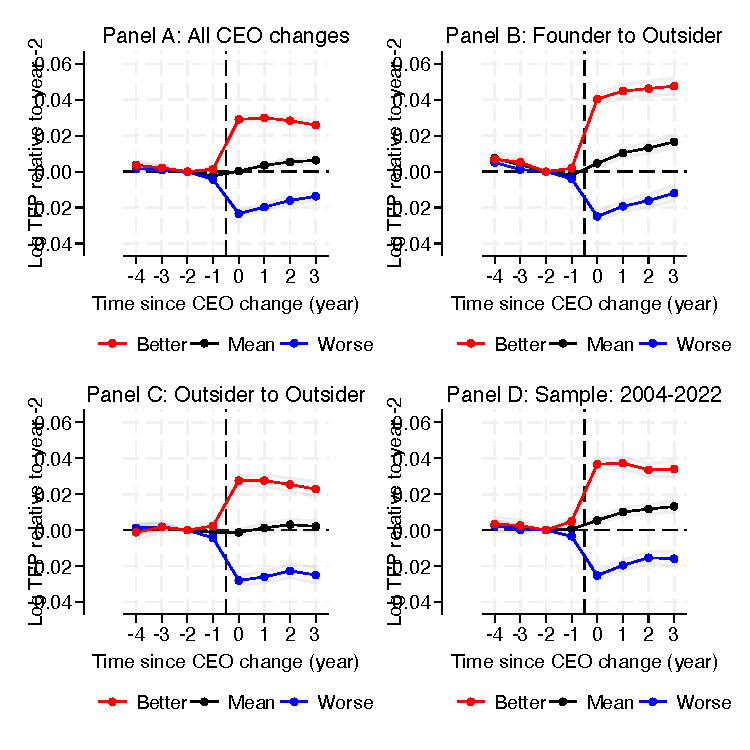
\includegraphics[width=\textwidth]{figure/figure1.pdf}
\caption{Placebo-Controlled Event Studies of CEO Transitions}
\label{fig:event_study_main}
\end{figure}

Finally, we analyze perhaps the most interesting question: how the productivity reacts to the arrival of a better or worse CEO than the incumbent? For this, we split the sample into two types of CEO transitions: when the incoming CEO has a higher or lower quality (as measured by the associated fixed effect) than the incumbent CEO. We also split the placebo sample into firms which experience an increase/decline of their TFP around the pseudo CEO change. The estimated coefficients are presented in the last two columns of Table \ref{tab:placeholder} and demonstrate the importance of CEOs and also show how the placebo correction works. Better CEOs than the incumbent increase TFP by 6\% while worse CEOs decrease it by 5\%. This large effect, however, is upward biased, as the placebo regressions demonstrate. The pseudo CEO change also produces a sizable effect of $\pm$2.5\%. Thus, the corrected effect is much smaller: better CEOs increase TFP by 2.7\% while worse CEOs decrease it by 1.8\%. Thus, the difference between a good and a bad CEO is 4.5\%. 

Figure \ref{fig:event_study_main} visualizes the evolution of TFP around the CEO change for four samples: all changes, when the incumbent is the founder of the firm, all other incumbents, and for the period of mature market economy (2004 -- 2022).\footnote{The latter sample is used to make our results more comparable to mature market economies. In the 1990s the economy was changing rapidly as it underwent rapid economic liberalization, transition to market economy, foreign direct investment inflows and large scale privatization. We conduct this robustness check by restricting the sample to post-2004 data following Hungary's EU accession.} On each figure we present the event time regression estimates for the whole sample (black line) and for better and worse CEO replacements (blue and red lines). The estimations leave little pre-trend and we find large swings in TFP. If the incoming CEO is better than the incumbent, TFP increases by 3 -- 4\% while worse CEOs decrease it by about 2\%. New CEOs have an effect immediately on the firm and this proves to be quite stable, as the estimated coefficients do not change much.  

\begin{figure}[htbp]
\centering
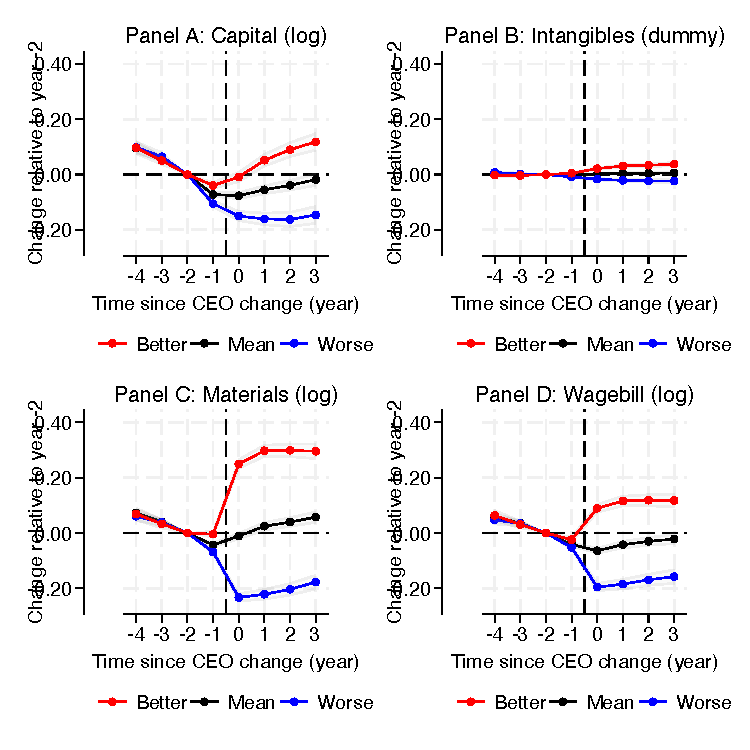
\includegraphics[width=\textwidth]{figure/figure2.pdf}
\caption{Placebo-Controlled Event Studies of CEO Transitions. Effects on Firm Inputs}
\label{fig:event_study_input}
\end{figure}

\paragraph{Model Validation: Differential Effects on Short- and Long-Term Inputs.} Our model predicts that CEOs should primarily affect outcomes they control (labor, materials) rather than those controlled by owners (capital, organizational structure). Figure \ref{fig:event_study_input} presents event studies for owner-controlled inputs (fixed assets and intangibles) and manager-controlled inputs (employment and materials).

Good CEOs have immediate and substantial effects on manager-controlled inputs. Material costs increase by 30\% and the wage bill by 13 percent (all effects highly significant). Firms under bad managers experience the opposite: a decline in material and employment costs by about 20\%. These effects appear immediately in the year of CEO transition and persist throughout the post-period, consistent with new CEOs quickly adjusting operational scale.

In contrast, owner-controlled variables show different patterns. Fixed assets exhibit a gradual change under good CEOs and little or no change under bad CEOs. The proportion of firms with intangible assets does not change at all around the CEO transition.

\paragraph{Contribution of CEOs to Firm Productivity.} To assess how important CEOs are for firm performance, we conduct the variance decomposition. As we describe at the end of Section \ref{sec:est}, we face two challenges. The variance is biased and it also depends on firm age. The outcome of our method is presented in Figure \ref{fig:variance_decomp} for TFP in the top row and log revenue in the bottom row. The blue line shows the within-firm change in variance relative to the second year after firm foundation. The blue line on panels A and C show the evolution of this variance around the CEO transition. Before the CEO transition, the variance grows continuously. The transition increases the variance abruptly; in later years it stays relatively stable for TFP and continues growing for revenue. Part of this growth, however, is due to limited mobility bias, and part arises mechanically: as time passes, the chance of receiving shocks increases. To control for these biases, we estimate the same variance on the pseudo transition sample. As the red line shows, this also increases in time. Panels B and D of the figure show the evolution of the estimated variance in the two samples by firm age. 

Our estimate of the contribution of CEO change to the total variance of TFP is the difference between the two estimates, and we quantify it in Appendix Table \ref{tab:var_share}. The table presents the total variance, the unadjusted contribution of CEO change and the adjusted contribution. We analyze only one CEO change, and the contribution depends on the length of the period measured (the longer the period, the more the variance increases for reasons unrelated to CEO change). In the first 10 years of existence, the uncorrelated share of CEO change in the variance is 62\%. Our correction decreases this number to 29\%.


\begin{figure}[htbp]
\centering
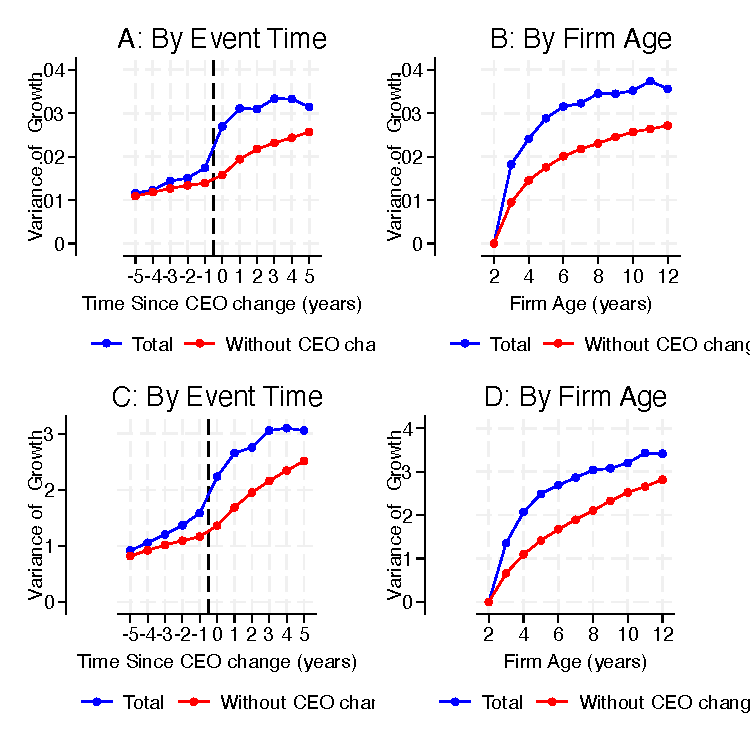
\includegraphics[width=\textwidth]{figure/figure3.pdf}
\label{fig:variance_decomp}
\begin{minipage}{15cm}
\caption{Decomposition of the Variance}
\vspace{.2cm}
\footnotesize Notes: Dependent variable: TFP (panels A and B), Log Revenue (panels C and D). Panels A and C present the variance growth relative to the year after firm foundation for firms with a CEO transition (blue line) and with a pseudo transition (red line). Panels B and D show the evolution of the variance in treated and pseudo-treated firms by firm age. 
\end{minipage}
\end{figure}

%%%%%%%%%%%%%%%%%%%%
\section{Conclusion}
%%%%%%%%%%%%%%%%%%%%

This paper estimates the contribution of CEOs to firm productivity by exploiting a unique administrative dataset covering the entire population of Hungarian private firms and their CEOs from 1992 to 2022. The novelty of the data lies in its unprecedented scope and completeness, allowing the study of CEO effects not only in large firms but crucially in small and medium-sized enterprises that dominate every economy. The combination of the dataset with a theoretically grounded model that distinguishes owner-controlled capital decisions from CEO-controlled operational inputs allows for a more precise attribution of productivity effects. 

The paper develops a new placebo-controlled event study design that overcomes limited mobility bias, which contaminates studies using two fixed effects.  By creating matched placebo CEO transitions in firms without actual leadership changes, the method effectively separates true CEO skill effects on productivity from mechanical noise. Empirically, the findings reveal that the true causal effect of CEO quality on firm productivity is economically meaningful but notably smaller than raw correlations suggest, explaining about 7–8 percent of productivity variation. 

An alternative way to deal with the noise problem is to use observable manager characteristics as measures of skill. Observable characteristics such as education and work experience \citep{DePirro2025}, foreign name as a proxy for international exposure \citep{Koren2023expat}, and the selectiveness of entry cohorts \citep{koren2024managers} offer more reliable, though narrower, measures of specific dimensions of managerial quality. These observables capture only partial aspects of CEO ability but avoid the mechanical noise that contaminates fixed effects estimates.

\clearpage
\bibliographystyle{apalike}
\bibliography{references}

\clearpage
\appendix
\section{Online Appendix: Additional Tables and Figures}
\renewcommand{\thefigure}{A\arabic{figure}}
\renewcommand{\thetable}{A\arabic{table}}
\setcounter{figure}{0}
\setcounter{table}{0}

\begin{table}[htbp]
\centering
\caption{Sample Over Time}
\label{tab:sample}
\begin{tabular}{*{6}{c}}
\toprule
Year & \shortstack{Total\\firms} & \shortstack{Sample\\firms} & CEOs & \multicolumn{2}{c}{Connected component} \\
\cmidrule(lr){5-6}
 & & & & Firms & CEOs \\
\midrule
1992 &       98,780 &       25,833 &       31,746 &        1,423 &        1,713 \\
1995 &      171,759 &       45,828 &       53,704 &        2,659 &        3,028 \\
2000 &      280,386 &       73,837 &       83,862 &        4,783 &        5,100 \\
2005 &      326,905 &       92,242 &      104,380 &        6,283 &        6,474 \\
2010 &      384,570 &      103,892 &      116,680 &        7,405 &        7,084 \\
2015 &      433,371 &      116,543 &      124,960 &        8,332 &        7,488 \\
2020 &      424,501 &      115,755 &      123,504 &        7,789 &        6,841 \\
2022 &      454,106 &      113,387 &      121,730 &        7,419 &        6,509 \\
\midrule
Total &    1,063,172 &      217,737 &      339,993 &       14,416 &       22,001 \\
\bottomrule
\end{tabular}
\begin{minipage}{12cm}
\footnotesize
\textit{Notes:} This table presents the evolution of the sample from 1992 to 2022. Column (1) shows the total number of distinct firms with balance sheet data. Column (2) shows the number of distinct firms after applying data quality filters. Column (3) shows the number of distinct CEOs. Columns (4) and (5) show the subset of distinct firms and CEOs that belong to the largest connected component of the manager network, where managers are connected if they have worked at the same firm. The table shows every fifth year plus the first year (1992), last year (2022), and totals of distinct counts. \end{minipage}
\end{table}


\begin{table}[htbp]
\centering
\caption{Industry Breakdown}
\label{tab:industry_stats}
\begin{tabular}{l*{5}{r}}
\toprule
Industry (NACE) & \shortstack{Obs.} & \shortstack{Firms} & \shortstack{CEOs} & \shortstack{Surplus\\share (\%)} \\
\midrule
Agriculture, Forestry, Fishing (A) &      320,485 &       25,951 &       55,535 &   7.9 \\
Manufacturing (C) &    1,022,252 &       90,035 &      179,205 &  13.7 \\
Wholesale, Retail, Transportation (G,H) &    2,887,229 &      296,237 &      550,110 &   6.4 \\
Telecom, Business Services (J,M) &    1,968,969 &      186,013 &      345,304 &  18.8 \\
Construction (F) &      962,938 &      112,633 &      183,144 &  11.4 \\
Nontradable Services (Other) &    2,775,169 &      277,749 &      527,661 &  13.5 \\
Mining, Quarrying (B)* &       13,428 &        1,151 &        2,922 &  23.8 \\
Finance, Insurance, Real Estate (K,L)* &      201,527 &       22,344 &       48,153 &  48.0 \\
\bottomrule
\end{tabular}
\begin{minipage}{\textwidth}
\footnotesize
\textit{Notes:} This table presents industry-level summary statistics using the TEAOR08 classification system. Column (1) shows the industry name and corresponding NACE sector codes. Column (2) shows the total number of firm-year observations in the balance sheet data (1992-2022). Column (3) shows the number of distinct firms with balance sheet data. Column (4) shows the number of distinct managers (CEOs) from the firm registry data. Column (5) shows the average EBITDA as a percentage of revenue. Mining (sector B) and Finance/Insurance/Real Estate (sectors K,L) are excluded from the main analysis due to different production function characteristics. The NACE classification follows the Hungarian adaptation of the NACE Rev. 2 system. \end{minipage}
\end{table}

%Benne maradhat a populáció, de kellene a minta is. Esetleg kidobhatjuk a firms oszlopot, és készítsük el a táblát a populációra és a mi mintánkra (Population: firm-year CEO, Sample: firm-year CEO, Surplus Share)


%\begin{table}[htbp]\centering
\def\sym#1{\ifmmode^{#1}\else\(^{#1}\)\fi}
\caption{Surplus Function Estimation Results}
\begin{tabular}{l*{6}{c}}
\toprule
                    &\multicolumn{1}{c}{(1)}&\multicolumn{1}{c}{(2)}&\multicolumn{1}{c}{(3)}&\multicolumn{1}{c}{(4)}&\multicolumn{1}{c}{(5)}&\multicolumn{1}{c}{(6)}\\
                    &\multicolumn{1}{c}{Revenue}&\multicolumn{1}{c}{EBITDA}&\multicolumn{1}{c}{Wagebill}&\multicolumn{1}{c}{Materials}&\multicolumn{1}{c}{Revenue}&\multicolumn{1}{c}{Revenue}\\
\midrule
Fixed assets (log)  &       0.323\sym{***}&       0.325\sym{***}&       0.287\sym{***}&       0.375\sym{***}&       0.290\sym{***}&       0.295\sym{***}\\
                    &     (0.001)         &     (0.001)         &     (0.001)         &     (0.002)         &     (0.001)         &     (0.004)         \\
\addlinespace
Has intangible assets&       0.268\sym{***}&       0.163\sym{***}&       0.267\sym{***}&       0.317\sym{***}&       0.205\sym{***}&       0.255\sym{***}\\
                    &     (0.003)         &     (0.003)         &     (0.003)         &     (0.004)         &     (0.003)         &     (0.010)         \\
\addlinespace
Founding owner      &      -0.079\sym{***}&      -0.051\sym{***}&      -0.017\sym{***}&      -0.099\sym{***}&      -0.010\sym{***}&      -0.015\sym{*}  \\
                    &     (0.005)         &     (0.005)         &     (0.005)         &     (0.006)         &     (0.003)         &     (0.008)         \\
\addlinespace
Non-founding owner  &      -0.001         &      -0.000         &      -0.003         &      -0.006         &      -0.011\sym{***}&      -0.017\sym{*}  \\
                    &     (0.007)         &     (0.006)         &     (0.007)         &     (0.009)         &     (0.004)         &     (0.009)         \\
\addlinespace
Foreign owned       &       0.025\sym{**} &       0.018         &       0.064\sym{***}&       0.010         &       0.022\sym{*}  &       0.033         \\
                    &     (0.012)         &     (0.012)         &     (0.012)         &     (0.015)         &     (0.011)         &     (0.025)         \\
\addlinespace
State owned         &       0.148\sym{***}&       0.047\sym{*}  &       0.448\sym{***}&       0.146\sym{***}&       0.062\sym{**} &       0.050         \\
                    &     (0.029)         &     (0.028)         &     (0.029)         &     (0.032)         &     (0.026)         &     (0.059)         \\
\midrule
Observations        &     3004184         &     2326192         &     2949024         &     3059662         &     2967233         &      374084         \\
\bottomrule
\multicolumn{7}{l}{\footnotesize Standard errors in parentheses}\\
\multicolumn{7}{l}{\footnotesize All models include firm fixed effects, industry-year fixed effects, and a step function for firm age.}\\
\multicolumn{7}{l}{\footnotesize Outcome variables are log-transformed. Models (5) and (6) include quadratic controls for CEO age and tenure.}\\
\multicolumn{7}{l}{\footnotesize Model (6) restricts to largest connected component of CEO-firm network.}\\
\multicolumn{7}{l}{\footnotesize \sym{*} \(p<0.10\), \sym{**} \(p<0.05\), \sym{***} \(p<0.01\)}\\
\end{tabular}
\end{table}



\begin{table}[htbp]
\centering
\caption{Share of Variance Attributed to CEO Change}
\vspace{.2cm}
\label{tab:var_share}
\begin{tabular}{lccc}
\toprule
Firm age & Total Variance Growth & Naive ANOVA share & Adjusted ANOVA share \\
\hline
4 &     0.024 &  0.544 &  0.451 \\
8 &     0.033 &  0.625 &  0.368 \\
12 &     0.035 &  0.620 &  0.269 \\ \bottomrule
\end{tabular}
\begin{minipage}{14cm}
\vspace{.2cm}
\footnotesize \textit{Notes:} The table presents the total variance growth of TFP since the second full year after firm establishment (Column 1), the uncorrected contribution of CEO change to total variance growth (Column 2) and the corrected contribution (Column 3). 
\end{minipage}
\end{table}



\end{document}








\appendix
\section{Online Appendix: Additional Tables and Figures}
\renewcommand{\thefigure}{A\arabic{figure}}
\renewcommand{\thetable}{A\arabic{table}}
\setcounter{figure}{0}
\setcounter{table}{0}

\subsection{Production Manager Autonomy in Family Firms}

%\begin{table}[htbp]\centering
\def\sym#1{\ifmmode^{#1}\else\(^{#1}\)\fi}
\caption{Plant Manager Autonomy in Family-Controlled Firms}
\begin{tabular}{l*{5}{c}}
\toprule
                    &\multicolumn{1}{c}{(1)}&\multicolumn{1}{c}{(2)}&\multicolumn{1}{c}{(3)}&\multicolumn{1}{c}{(4)}&\multicolumn{1}{c}{(5)}\\
                    &\multicolumn{1}{c}{Investment}&\multicolumn{1}{c}{Investment}&\multicolumn{1}{c}{Marketing}&\multicolumn{1}{c}{Product}&\multicolumn{1}{c}{Hiring}\\
\midrule
Family ownership    &      -0.369\sym{**} &      -0.200\sym{**} &      -0.344\sym{**} &      -0.299\sym{**} &       0.086         \\
                    &     (0.161)         &     (0.100)         &     (0.153)         &     (0.151)         &     (0.068)         \\
\midrule
Observations        &       2,915         &       2,379         &       3,133         &       3,114         &       3,138         \\
Country FE          &         Yes         &         Yes         &         Yes         &         Yes         &         Yes         \\
Industry FE         &         Yes         &         Yes         &         Yes         &         Yes         &         Yes         \\
\bottomrule
\multicolumn{6}{l}{\footnotesize Standard errors in parentheses}\\
\multicolumn{6}{l}{\footnotesize Data source: Bloom, Sadun, and Van Reenen (2012). Sample restricted to private (non-publicly traded) firms.}\\
\multicolumn{6}{l}{\footnotesize Investment autonomy measured as maximum capital investment plant manager can approve (USD).}\\
\multicolumn{6}{l}{\footnotesize Other autonomy dimensions are binary indicators for full autonomy (score = 5 on 1-5 scale).}\\
\multicolumn{6}{l}{\footnotesize PPML = Poisson Pseudo-Maximum Likelihood. Standard errors clustered at firm level.}\\
\multicolumn{6}{l}{\footnotesize All specifications include country and 2-digit SIC industry fixed effects.}\\
\multicolumn{6}{l}{\footnotesize \sym{*} \(p<0.10\), \sym{**} \(p<0.05\), \sym{***} \(p<0.01\)}\\
\end{tabular}
\end{table}


\subsection{Industry Breakdown}

%\begin{table}[htbp]
\centering
\caption{Sample Over Time}
\label{tab:sample}
\begin{tabular}{*{6}{c}}
\toprule
Year & \shortstack{Total\\firms} & \shortstack{Sample\\firms} & CEOs & \multicolumn{2}{c}{Connected component} \\
\cmidrule(lr){5-6}
 & & & & Firms & CEOs \\
\midrule
1992 &       98,780 &       25,833 &       31,746 &        1,423 &        1,713 \\
1995 &      171,759 &       45,828 &       53,704 &        2,659 &        3,028 \\
2000 &      280,386 &       73,837 &       83,862 &        4,783 &        5,100 \\
2005 &      326,905 &       92,242 &      104,380 &        6,283 &        6,474 \\
2010 &      384,570 &      103,892 &      116,680 &        7,405 &        7,084 \\
2015 &      433,371 &      116,543 &      124,960 &        8,332 &        7,488 \\
2020 &      424,501 &      115,755 &      123,504 &        7,789 &        6,841 \\
2022 &      454,106 &      113,387 &      121,730 &        7,419 &        6,509 \\
\midrule
Total &    1,063,172 &      217,737 &      339,993 &       14,416 &       22,001 \\
\bottomrule
\end{tabular}
\begin{minipage}{12cm}
\footnotesize
\textit{Notes:} This table presents the evolution of the sample from 1992 to 2022. Column (1) shows the total number of distinct firms with balance sheet data. Column (2) shows the number of distinct firms after applying data quality filters. Column (3) shows the number of distinct CEOs. Columns (4) and (5) show the subset of distinct firms and CEOs that belong to the largest connected component of the manager network, where managers are connected if they have worked at the same firm. The table shows every fifth year plus the first year (1992), last year (2022), and totals of distinct counts. \end{minipage}
\end{table}


%\begin{table}[htbp]\centering
\def\sym#1{\ifmmode^{#1}\else\(^{#1}\)\fi}
\caption{The revenue function by sector}
\begin{tabular}{l*{6}{c}}
\hline\hline
                    &\multicolumn{1}{c}{(1)}&\multicolumn{1}{c}{(2)}&\multicolumn{1}{c}{(3)}&\multicolumn{1}{c}{(4)}&\multicolumn{1}{c}{(5)}&\multicolumn{1}{c}{(6)}\\
                    &\multicolumn{1}{c}{Agriculture}&\multicolumn{1}{c}{Manufacturing}&\multicolumn{1}{c}{Wholesale, Retail, Transportation}&\multicolumn{1}{c}{Telecom and Business Services}&\multicolumn{1}{c}{Construction}&\multicolumn{1}{c}{Nontradable services}\\
\hline
Tangible and intangible assets (log)&       0.320\sym{***}&       0.296\sym{***}&       0.257\sym{***}&       0.237\sym{***}&       0.281\sym{***}&       0.207\sym{***}\\
                    &     (0.006)         &     (0.003)         &     (0.002)         &     (0.002)         &     (0.002)         &     (0.002)         \\
[1em]
Intangible assets share&       0.071         &       0.011         &      -0.006         &      -0.057\sym{***}&       0.029         &      -0.020         \\
                    &     (0.059)         &     (0.025)         &     (0.014)         &     (0.013)         &     (0.030)         &     (0.015)         \\
[1em]
Foreign owned       &      -0.070\sym{*}  &       0.046\sym{*}  &       0.008         &       0.082\sym{***}&      -0.055         &      -0.013         \\
                    &     (0.042)         &     (0.024)         &     (0.015)         &     (0.022)         &     (0.041)         &     (0.015)         \\
\hline
Observations        &      208269         &      748880         &     1893882         &     1224209         &      630073         &     1708957         \\
\hline\hline
\multicolumn{7}{l}{\footnotesize Controls: firm-CEO-spell fixed effects; industry-year fixed effects.}\\
\end{tabular}
\end{table}



\subsection{Manager Skill Distributions}

\begin{figure}[htbp]
\centering
\begin{minipage}{0.48\textwidth}
\centering
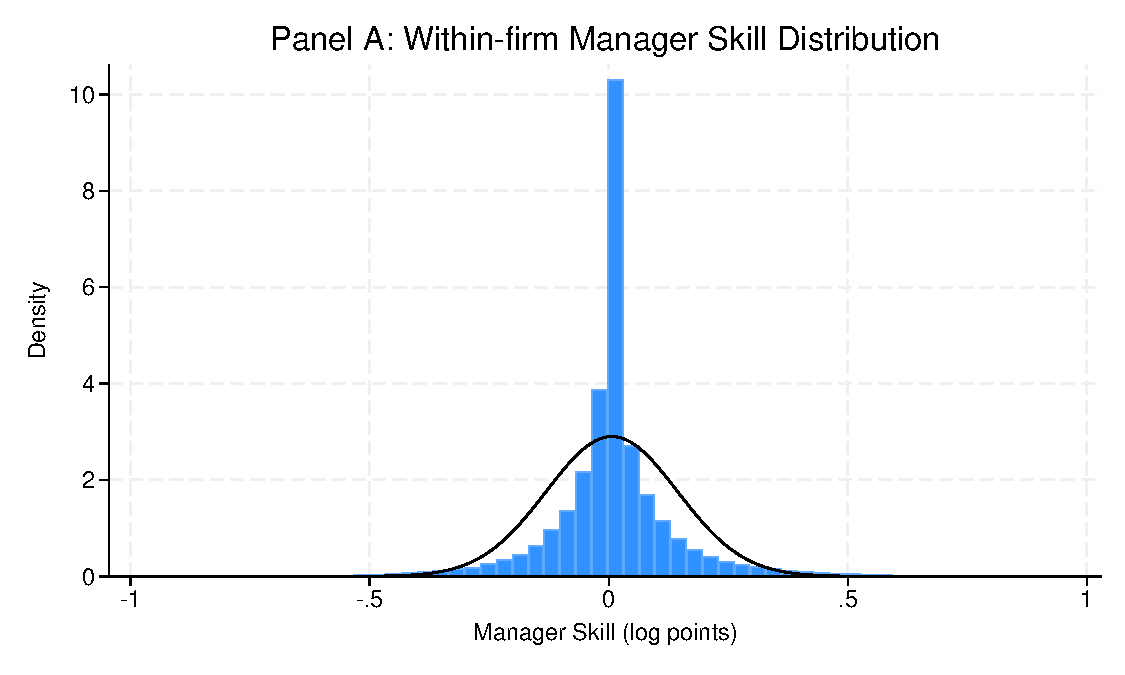
\includegraphics[width=\textwidth]{figure/manager_skill_within.pdf}
\end{minipage}
\hfill
\begin{minipage}{0.48\textwidth}
\centering
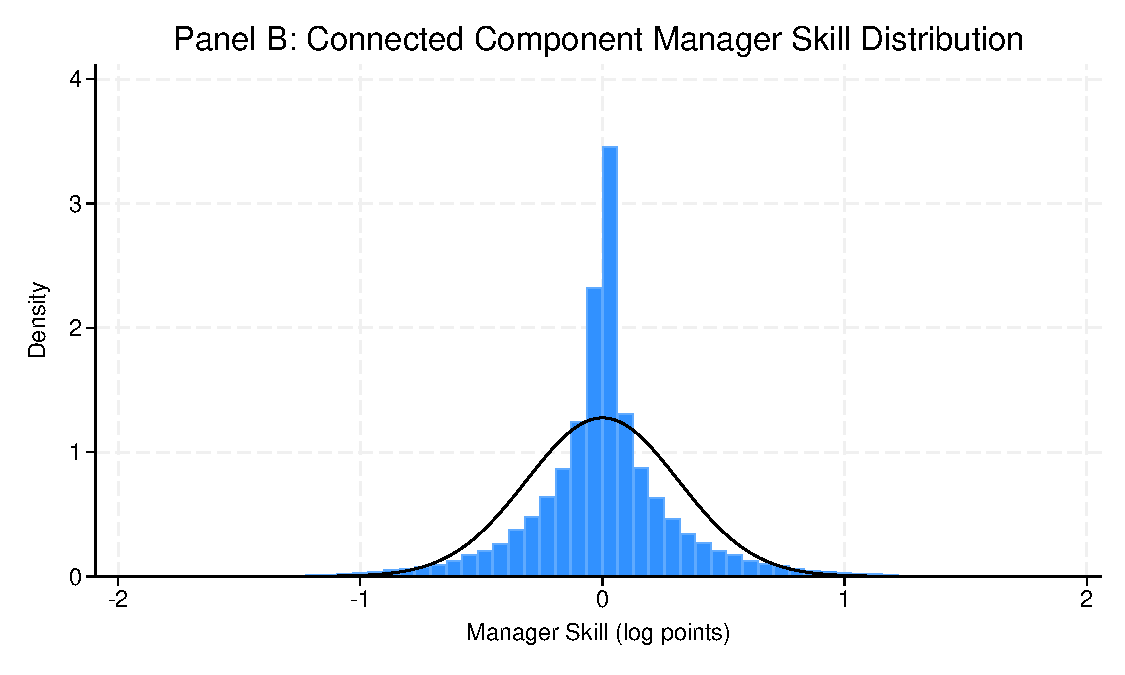
\includegraphics[width=\textwidth]{figure/manager_skill_connected.pdf}
\end{minipage}
\caption{Manager Skill Distributions}
\label{fig:manager_skills_appendix}
\footnotesize
Notes: Panel A shows the distribution of within-firm manager skill variation for firms with multiple CEOs. Panel B shows the distribution of manager skills in the largest connected component of managers. Both distributions show manager skills in log points after normalization and scaling.
\end{figure}


% Additional tables and figures to be inserted here as needed

\subsection{Variance-Based Evidence for CEO Heterogeneity}

\begin{figure}[htbp]
\centering
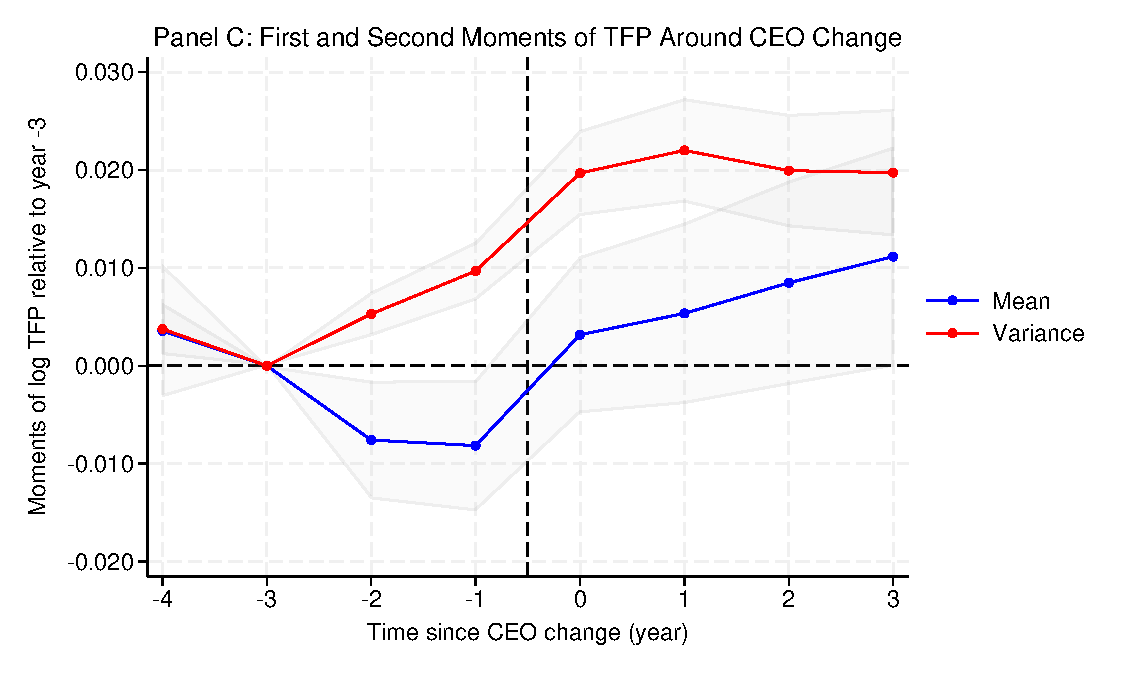
\includegraphics[width=0.8\textwidth]{figure/event_study_panel_c.pdf}
\caption{TFP Moments Around CEO Transitions}
\label{fig:intangibles}
\end{figure}

Figure \ref{fig:variance_event_study} presents complementary evidence using the variance of log TFP around CEO transitions. Under our framework, if CEO changes introduce real heterogeneity in managerial quality, the cross-sectional variance of outcomes should increase at the transition point—some firms get better CEOs, others get worse ones. In contrast, pure noise or firm-specific trends would not systematically alter variance.

The variance analysis shows that actual CEO transitions are associated with increased dispersion in outcomes, while placebo transitions show no such effect. This provides model-free evidence that CEO transitions introduce real heterogeneity in firm performance, supporting our identification strategy.


\subsection{Treatment Effects on Owner vs Manager Variables}

{
\def\sym#1{\ifmmode^{#1}\else\(^{#1}\)\fi}
\begin{tabular}{l*{3}{c}}
\hline\hline
                    &\multicolumn{1}{c}{(1)}&\multicolumn{1}{c}{(2)}&\multicolumn{1}{c}{(3)}\\
                    &\multicolumn{1}{c}{Fixed assets (log)}&\multicolumn{1}{c}{Has intangible assets}&\multicolumn{1}{c}{Foreign owned}\\
\hline
Better CEO          &       0.054         &       0.056\sym{***}&       0.051\sym{***}\\
                    &     (0.078)         &     (0.020)         &     (0.013)         \\
\hline
Observations        &       81272         &       81272         &       81272         \\
\hline\hline
\end{tabular}
}


{
\def\sym#1{\ifmmode^{#1}\else\(^{#1}\)\fi}
\begin{tabular}{l*{2}{c}}
\hline\hline
                    &\multicolumn{1}{c}{(1)}&\multicolumn{1}{c}{(2)}\\
                    &\multicolumn{1}{c}{Wagebill (log)}&\multicolumn{1}{c}{Materials (log)}\\
\hline
Better CEO          &       0.055\sym{***}&       0.127\sym{***}\\
                    &     (0.013)         &     (0.013)         \\
\hline
Observations        &     1089713         &     1089713         \\
\hline\hline
\end{tabular}
}

